%-------------------------------------------------------------
% Language
% Use the option "language=EN" to set the beamer theme in English. Use
% the option "language=ES" to set the beamer theme in Spanish.

% Colors
% Use the option "color=white" to set the background in white and the
% bottom bar in blue. Use the option "color=blue" to set the
% background in blue and the bottom bar in white. Use the option
% "color=blue2" to set the background in blue and the bottom bar in
% blue.

% Font Color
% Use the option "fontc=black" to set the font color in black. If this
% argument is not given the default color is set depending of the
% color scheme selected.

% Credits: https://github.com/alejogm0520 & Samuel Plazas Escudero
%-------------------------------------------------------------

%--Principal packages
\documentclass[aspectratio=43,8pt]{beamer} % 4:3, can be 16:9
\usetheme[language=ES, color=white]{EAFIT}
\usepackage[spanish]{babel}
\decimalpoint % All decimal numbers with point
\usepackage[utf8]{inputenc}
\selectlanguage{spanish}
\usepackage{amsmath,amsfonts,amssymb,cancel,physics} % Equations
\usepackage{verbatim} % Environments, \begin{comment}
%--Arial
\usepackage{helvet}
\renewcommand{\familydefault}{\sfdefault}
%--Beamer packages
\usepackage{tikz} % For making vectorized figures, arrows
\usepackage{ifthen} % For specifying conditionals for sections
\usepackage{ragged2e}\justifying % Whole text justified, except enumerate: add \justifying
\usepackage{xcolor}
\usepackage{multicol} % Multiple columns in one frame
%--Tables-Figures
\renewcommand\spanishtablename{Tabla}
\usepackage{booktabs,multirow} % Bookstyle tables
%-Figure label
\usepackage[labelsep=period,justification=justified,format=plain]{caption} % Dot instead of colon and justified caption
%--Figure
\usepackage{graphicx,subcaption} % Figures and subfigures
\graphicspath{{media/}} % Media rute
%-Figure-Table on top
\usepackage{float} % Allows to put H instead of ht
\setbeamertemplate{caption}[numbered] % Numbered captions
%---------TOC
\setbeamertemplate{section in toc}[sections numbered]
\setbeamertemplate{subsection in toc}[subsections numbered]
\setbeamerfont{section in toc}{size=\small}
\setbeamerfont{subsection in toc}{size=\footnotesize}
\setbeamertemplate{subsection in toc}{\leavevmode\leftskip=3.2em\rlap{\hskip-2em\inserttocsectionnumber.\inserttocsubsectionnumber}\inserttocsubsection\par} % Indented subsection
\setcounter{secnumdepth}{1}
%---------Cite
\usepackage{bibentry} % Full cite foot
\nobibliography* % Full cite foot
% Or: \setbeamertemplate{bibliography item}[text]
\setbeamertemplate{bibliography item}{\insertbiblabel}
%---------Footnotes
\setbeamercolor{footnote}{fg=white}
\setbeamercolor{footnote mark}{fg=.} % Takes the color depending on the circumpstance
\setbeamercolor{bibliography entry author}{fg=white} % Allows to have white footnote bibs
\setbeamertemplate{footnote}
{
  \hspace*{-1cm} % Horizontal movement
  \vspace*{-2.88cm} % Vertical movement
  \parbox[c][3.4cm]{10.6cm}{\tiny\noindent\insertfootnotemark\insertfootnotetext} % b: bottom, height: 3.3cm, horizontal length: 10.6cm (max horizontal)
% If there are problems, put -2.87cm and 3.3cm
}
\renewcommand{\footnoterule}{\kern -3pt \hrule width \textwidth height 0pt\kern 3pt} % No footnoterule
%------------------------------------
%---------Numbered Slides and Sections
\setbox0=\hbox{\subsecname\unskip}\ifdim\wd0=0pt\else%
 ~--~\insertsubsectionhead
\fi
%------Numbering section: title in bold, centered and with a line
\newcommand{\numb} 
{
  \setbeamertemplate{frametitle}
  {
    \ifx\insertsubsection\empty % No subsection
         \bfseries\thesection.~\insertframetitle~\color{black}\par\vskip-5pt\hrulefill % \centering
    \else % subsection
         \bfseries\thesection.~\insertframetitle~\color{black}\par\vskip-9pt\hrulefill\par\vskip3pt{\large\thesection.\thesubsection~\insertframesubtitle} % Subsection with smaller size;
    \fi
  }
}
%------No numbering section: title in bold, centered and with a line
\newcommand{\nonumb}
{
  \setbeamertemplate{frametitle}{\bfseries\color{black}\centering\insertframetitle\par\vskip-6pt\hrulefill}
}
%------------------------------------
%--No hyphenation on text
\tolerance=1
\emergencystretch=\maxdimen
\hyphenpenalty=10000
\hbadness=10000
%------------------------
%---------Itemize justified in beamer
\makeatletter
\renewcommand{\itemize}[1][]{
  \beamer@ifempty{#1}{}{\def\beamer@defaultospec{#1}}
  \ifnum \@itemdepth >2\relax\@toodeep\else
    \advance\@itemdepth\@ne
    \beamer@computepref\@itemdepth % Sets \beameritemnestingprefix
    \usebeamerfont{itemize/enumerate \beameritemnestingprefix body}
    \usebeamercolor[fg]{itemize/enumerate \beameritemnestingprefix body}
    \usebeamertemplate{itemize/enumerate \beameritemnestingprefix body begin}
    \list
      {\usebeamertemplate{itemize \beameritemnestingprefix item}}
      {\def\makelabel##1{
          {
            \hss\llap{{
                \usebeamerfont*{itemize \beameritemnestingprefix item}
                \usebeamercolor[fg]{itemize \beameritemnestingprefix item}##1}}
          }
        }
      }
  \fi
  \beamer@cramped
  \justifying % Justified itemize
  \beamer@firstlineitemizeunskip
}
\makeatother
%------------------------
%---------Get current section name for showing it at its begining
\usepackage{nameref}
\makeatletter
\newcommand*{\currentname}{\@currentlabelname}
\makeatother
%---------Shows in which section we are at the begining of each one
\AtBeginSection[]
{
\begin{frame}[plain,noframenumbering]
  \begin{beamercolorbox}[ht=\paperheight,wd=\paperwidth, center]{Portada}
    \begin{center}\textbf{\LARGE \currentname}\end{center} % Leave the next space mandatorily

    \vspace{0.44\paperheight}
  \end{beamercolorbox}
\end{frame}
}
%-------------------(constantly being edited)------------------

%---------TEXTBLOCKS-GRID 
\usepackage[absolute,overlay,showboxes]{textpos}
%\usepackage[texcoord,grid,gridunit=mm,gridcolor=red!10,subgridcolor=green!10]{eso-pic} % Helping grids, comment when publishing
%---------COLOR DEFINITIONS
\definecolor{azure(colorwheel)}{rgb}{0.0, 0.5, 1.0} % Define colors here


%%%%%%%%%%%%%%%%%%%%%%%
%Start of the Document%
%%%%%%%%%%%%%%%%%%%%%%%

%---------COVER PAGE

\title{CRIPTOGRAFÍA{}}
\author{\normalfont\large\texorpdfstring{Presentado por:\\ Juan S. Cárdenas Rodríguez\\  David Plazas Escudero}{}} % PA
\def\carrera{Ingeniería Matemática}
\def\departamento{Departamento de Ciencias Matemáticas}
\def\escuela{Escuela de Ciencias}
\def\materia{Modelación y Simulación II}
\def\eafit{Universidad EAFIT}
\def\fecha{2017}
% to add more def, search for "Dirección" in beamerthemeEAFIT.sty



%\includeonly{c/ex}
\begin{document}

\nonumb % Not numbered titles
\begin{frame}
% Portada Inspira Crea Transforma
\end{frame}
%%%%%%%%%%%%%%%%%%%%%%%%%%%%%%%%%%%%%%%%%%%%%%%%%%%%%%%%%%%%%%%%%%%%%%%%%%%%
\begin{frame}
\begin{center}
  \titlepage % Cover page
\end{center}
\end{frame}
%%%%%%%%%%%%%%%%%%%%%%%%%%%%%%%%%%%%%%%%%%%%%%%%%%%%%%%%%%%%%%%%%%%%%%%%%%%%
\begin{frame}{CONTENIDO}
\begin{multicols}{2}
  \tableofcontents
\end{multicols}
\end{frame}
\numb % Numbered titles
\section{DEFINICIÓN}
\begin{frame}{DEFINICIÓN}
	Es el cifrado y descifrado de mensajes  secretos o encriptados. También referido a encriptado computacional de información \vspace{-0.8cm}\footnote{\bibentry{defCrip}}. \footnotetext{\bibentry{imgDef}} \vspace{1cm}
    \begin{figure}[H]
    	\centering
        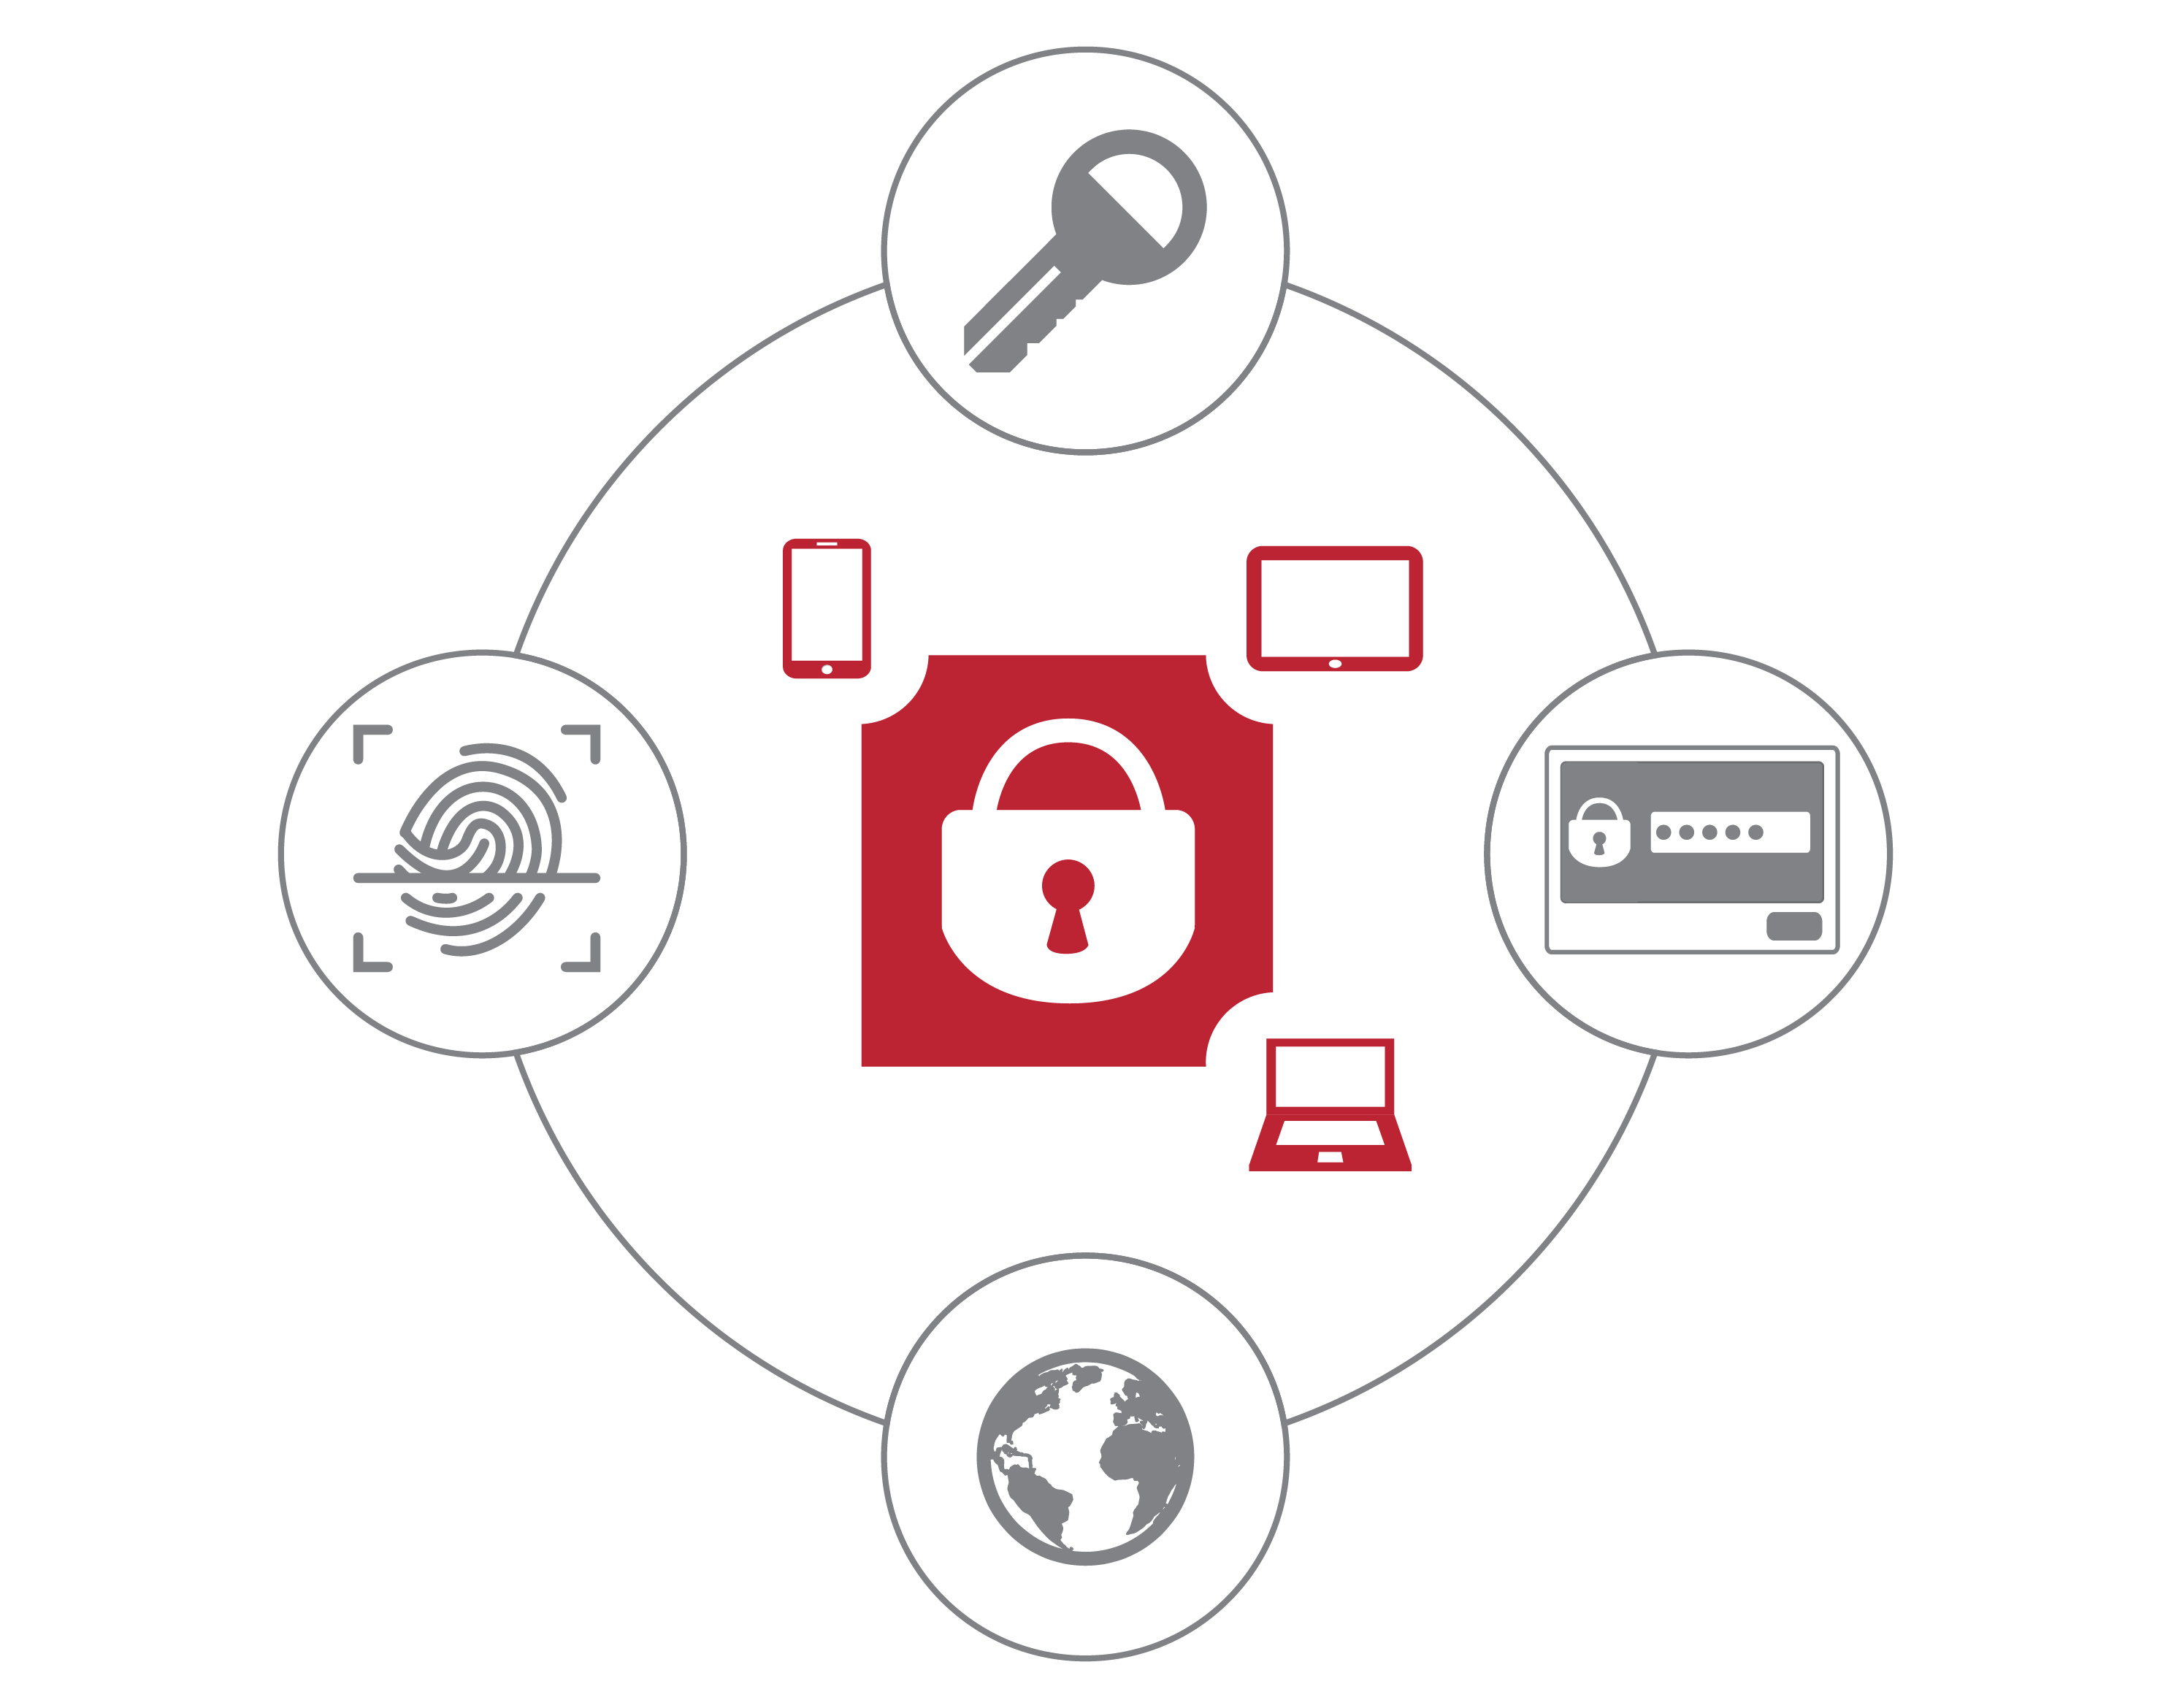
\includegraphics[scale=0.25]{def.png}
    \end{figure}
\end{frame}
\section{HISTORIA DE LA CRIPTOGRAFÍA}
\begin{frame}{HISTORIA DE LA CRIPTOGRAFÍA}
	\begin{itemize}
	\item Khnumhotep II - Egipto, India.
	\item Cifrado de César, 100 A.C.
	\item Cifrado de Vigenere, Siglo 16.
	\item La máquina Enigma.
	\end{itemize}
    \centering 158,962,555,217,826,360,000 
    \begin{figure}
    	\centering
        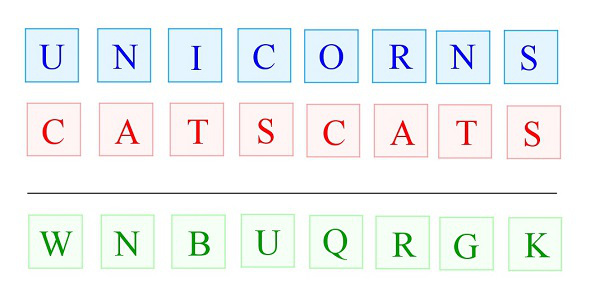
\includegraphics[scale=0.5]{vieCip.jpg}
        \caption{Ejemplo del Cifrado de Vigenere\footnotemark{}}
    \end{figure}
    \vspace{-3mm}\footnotetext{\bibentry{vige}}
\end{frame}
%%%%%%%%%%%%%%%%%%%%%%%%%%%%%%%%%%%%%%%%%%%%%%%%%%%%
\section{TIPOS DE CRIPTOGRAFÍA}
\subsection{Simétrica}
\begin{frame}{TIPOS DE CRIPTOGRAFÍA}
	\framesubtitle{Simétrica}
    Se utiliza la misma llave (privada) para cifrar y descifrar el mensaje.
    \begin{figure}
    	\centering
        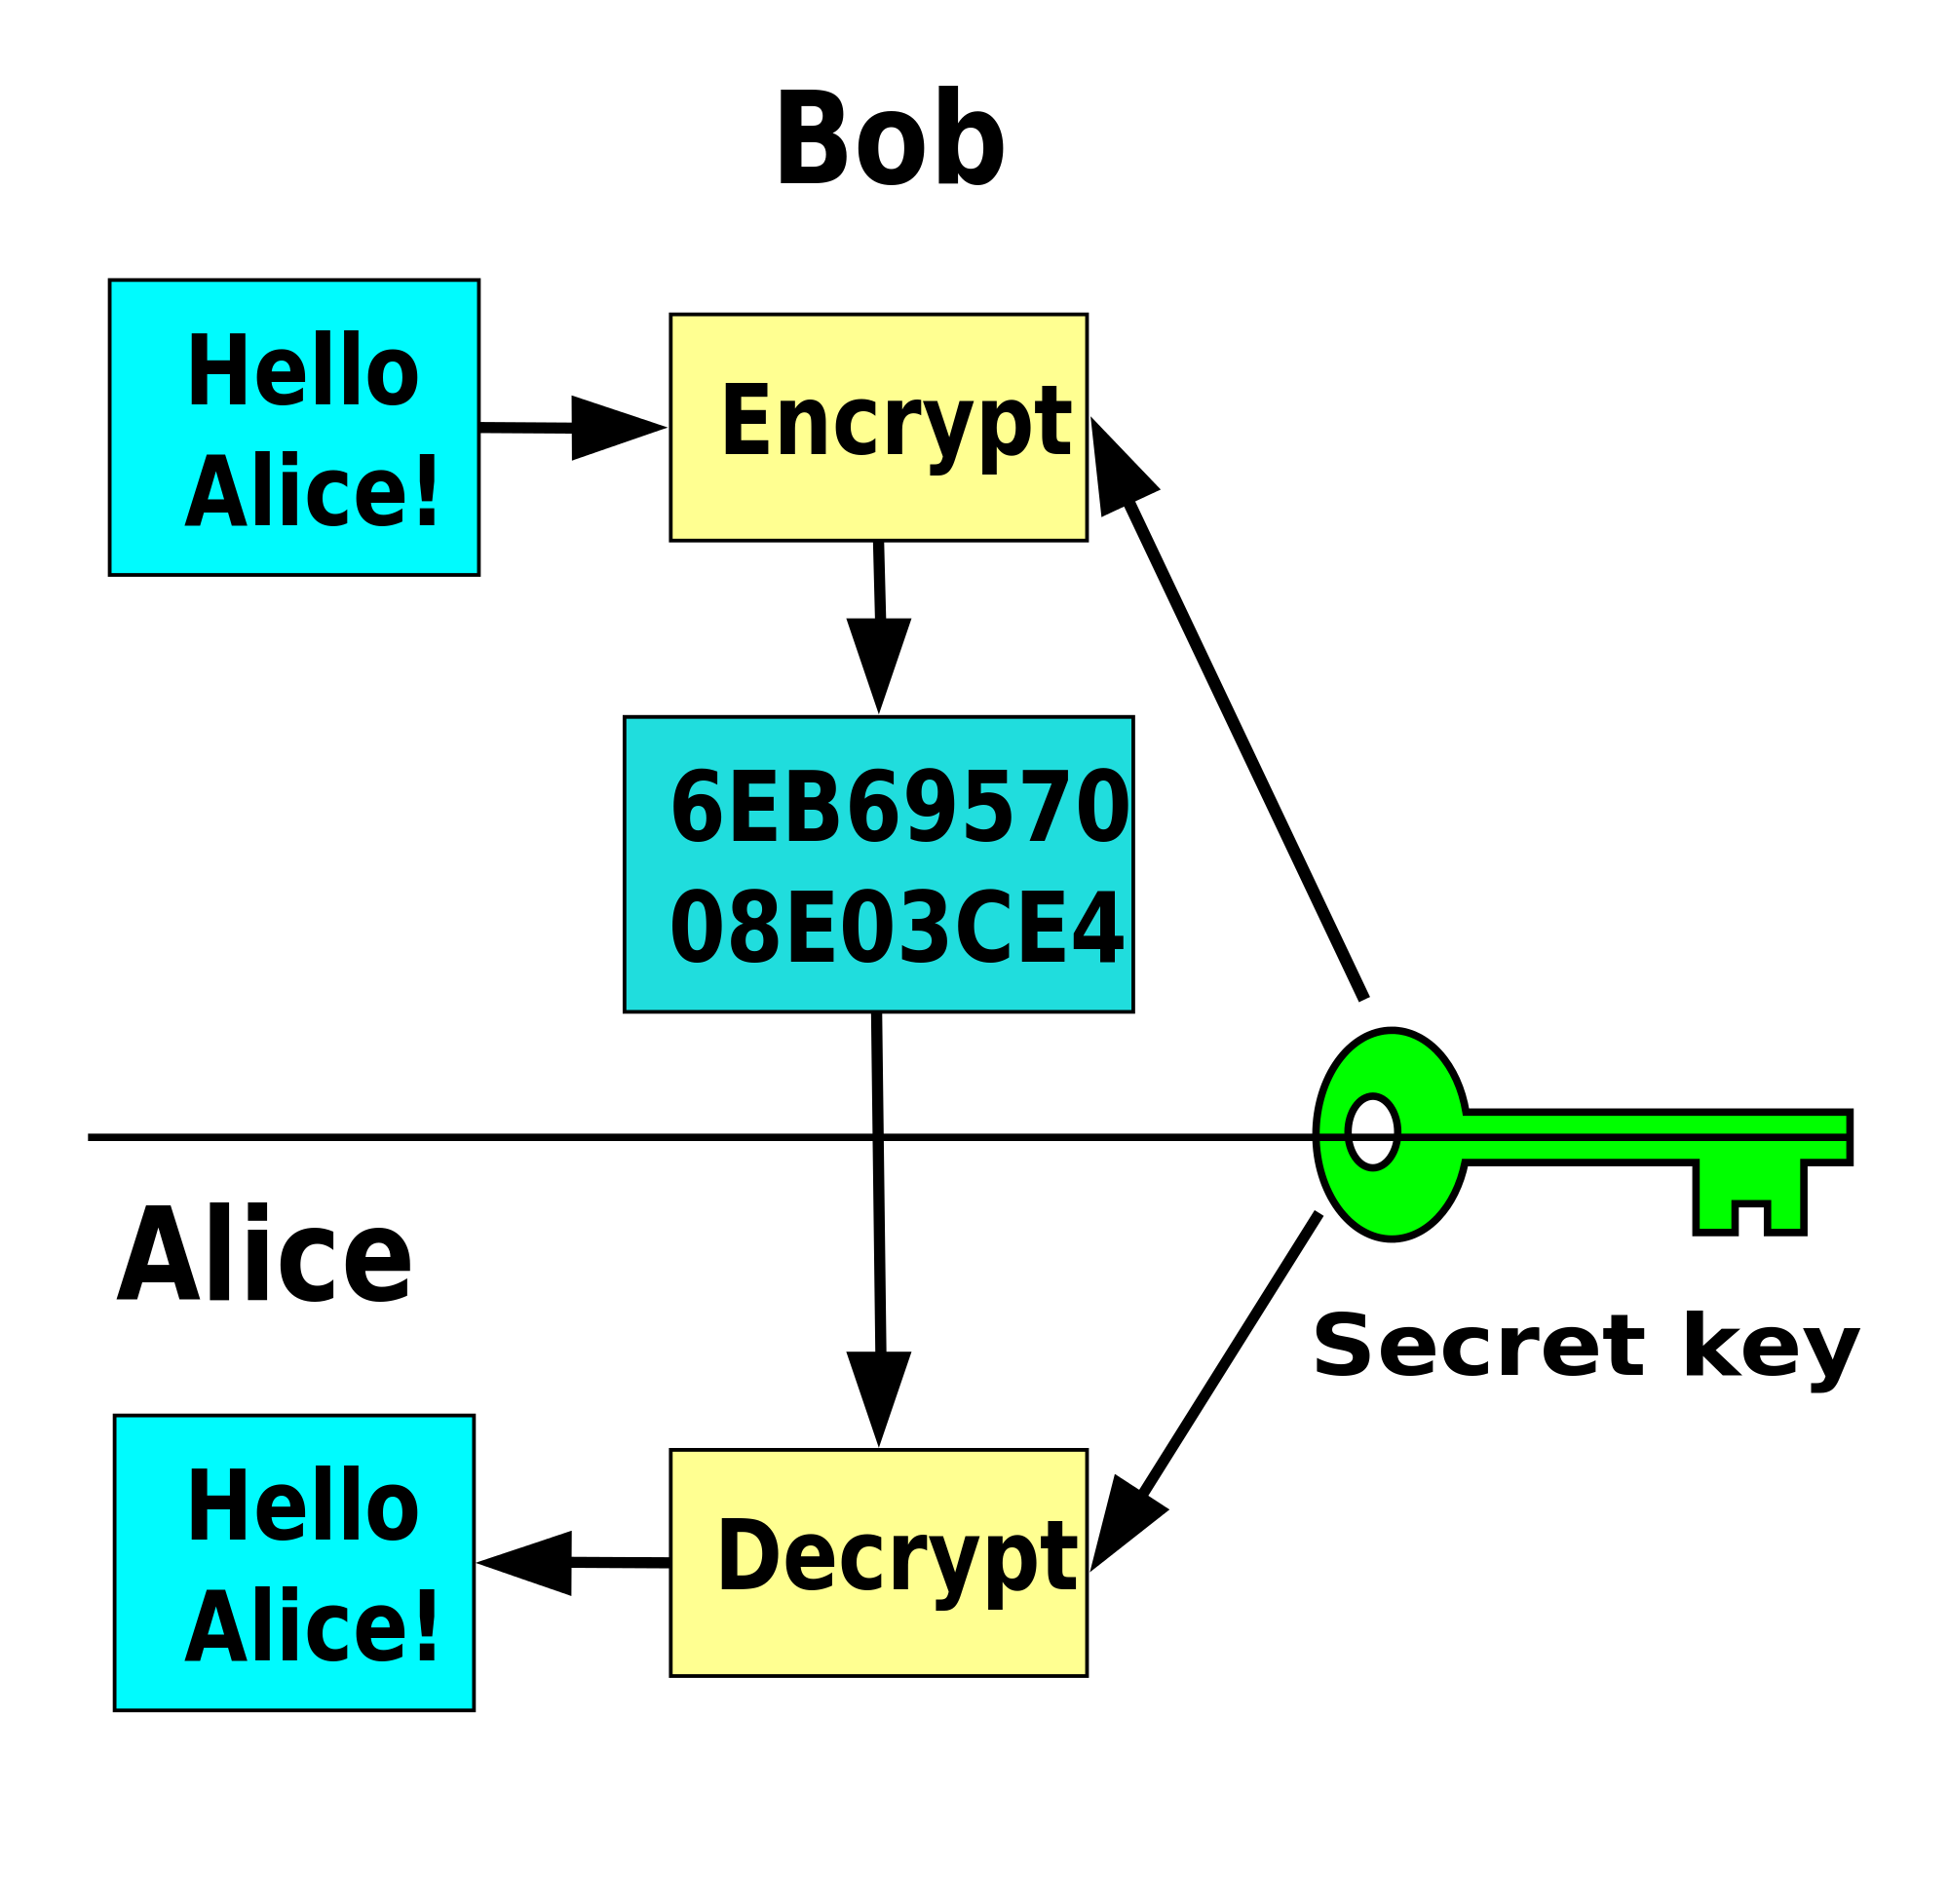
\includegraphics[scale=0.075]{symmetric.png}
        \caption{Ilustración de criptografía simétrica\footnotemark{}}
    \end{figure}
    \vspace{-0.5cm}\footnotetext{\bibentry{symm}}
\end{frame}
%%%%%%%%%%%%%%%%%%%%%%%%%%%%%%%%%%%%%%%%%%%%%%%%%%%%%
\subsection{Antisimétrica}
\begin{frame}{TIPOS DE CRIPTOGRAFÍA}
	\framesubtitle{Antisimétrica}
    Hay dos llaves, una privada y otra pública. Se puede utilizar la pública para encriptar la información o la privada para firmarla.
    \begin{figure}
    	\centering
        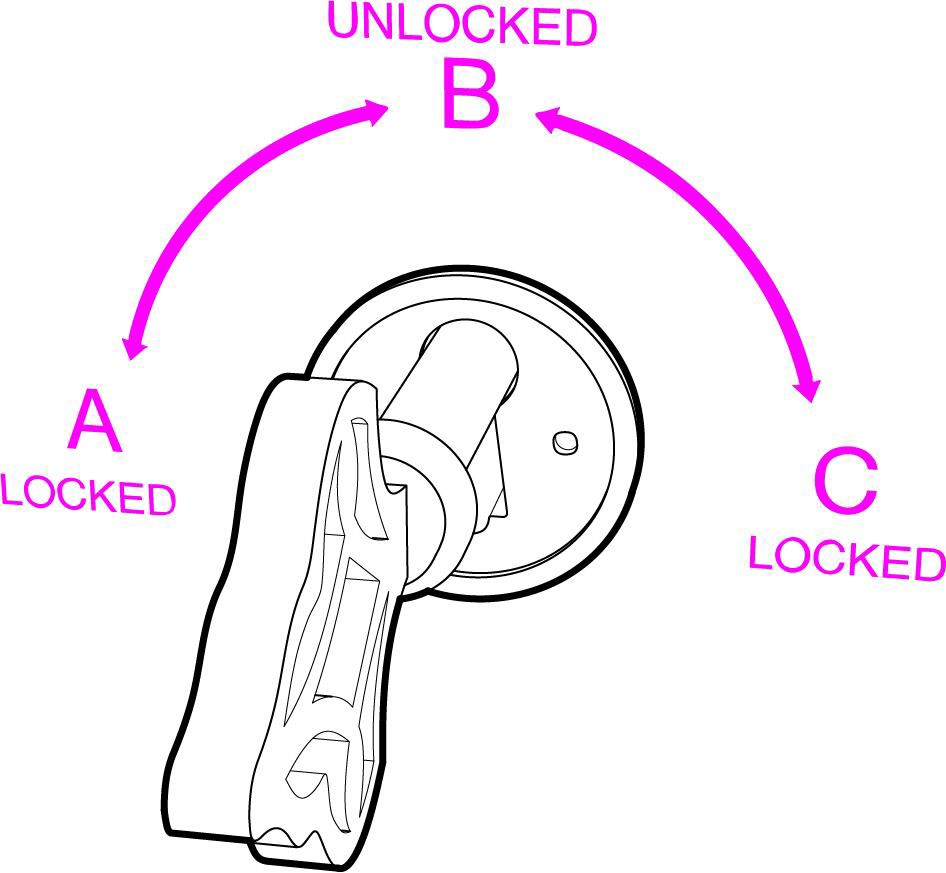
\includegraphics[scale=0.1]{lockUnlock.jpg}
        \caption{Ilustración de criptografía asimétrica\footnotemark{}}
    \end{figure}
    \footnotetext{\bibentry{lockU}}
\end{frame}

\section{NÚMEROS PRIMOS}
\subsection{Teoría}
\begin{frame}{NÚMEROS PRIMOS}
	\framesubtitle{Teoría}
	\begin{itemize}
      \item Teorema Fundamental de la aritmética
      \item ¿Cuántos primos hay en el intervalo (1,x)?
      \item Teorema de Chebyshev
      \item Problemas clásicos de los primos
	\end{itemize}
    \begin{figure}
    	\centering
        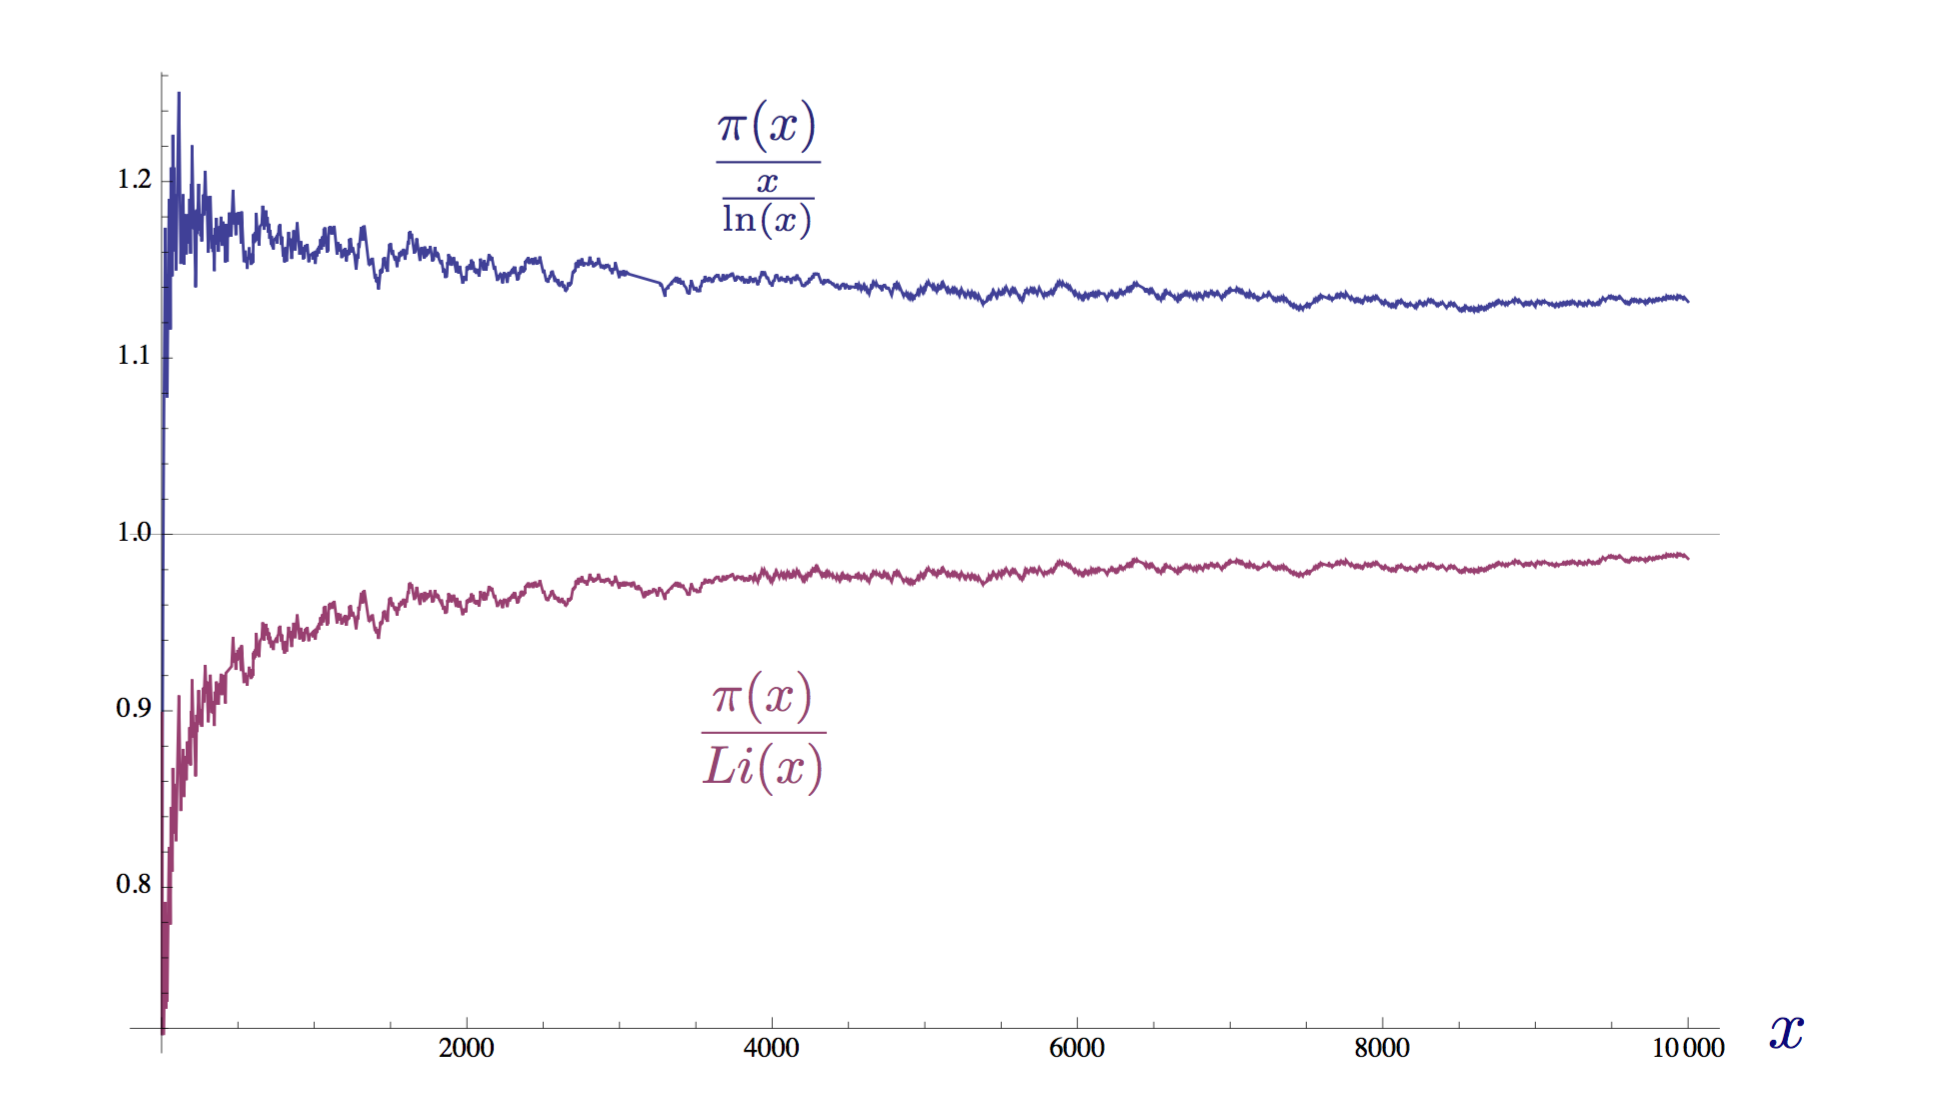
\includegraphics[scale=0.1]{ratioConv.png}
        \caption{Convergencia de la función contadora de primos a 1 por dos aproximaciones\footnotemark{}.}
    \end{figure}
    \vspace{-1cm}\footnotetext{\bibentry{conv}}
\end{frame}
%%%%%%%%%%%%%%%%%%%%%%%%%%%%%%%%%%%%%%%%%%%%%%%%%%%%%%%%%%
\subsection{Adicional}
\begin{frame}{NÚMEROS PRIMOS}
	\framesubtitle{Adicional}
    \begin{itemize}
    \item Función Zeta de Riemann
    	\begin{equation}
    		\zeta (s)=\sum_{n=1}^{\infty}{\frac{1}{n^s}}
    	\end{equation}
    \item Identidad de Euler
    	\begin{equation}
    		\zeta(s)=\prod_{p}{\frac{1}{1-p^{-s}}}
    	\end{equation}
    \end{itemize}
    \begin{figure}
    	\centering
        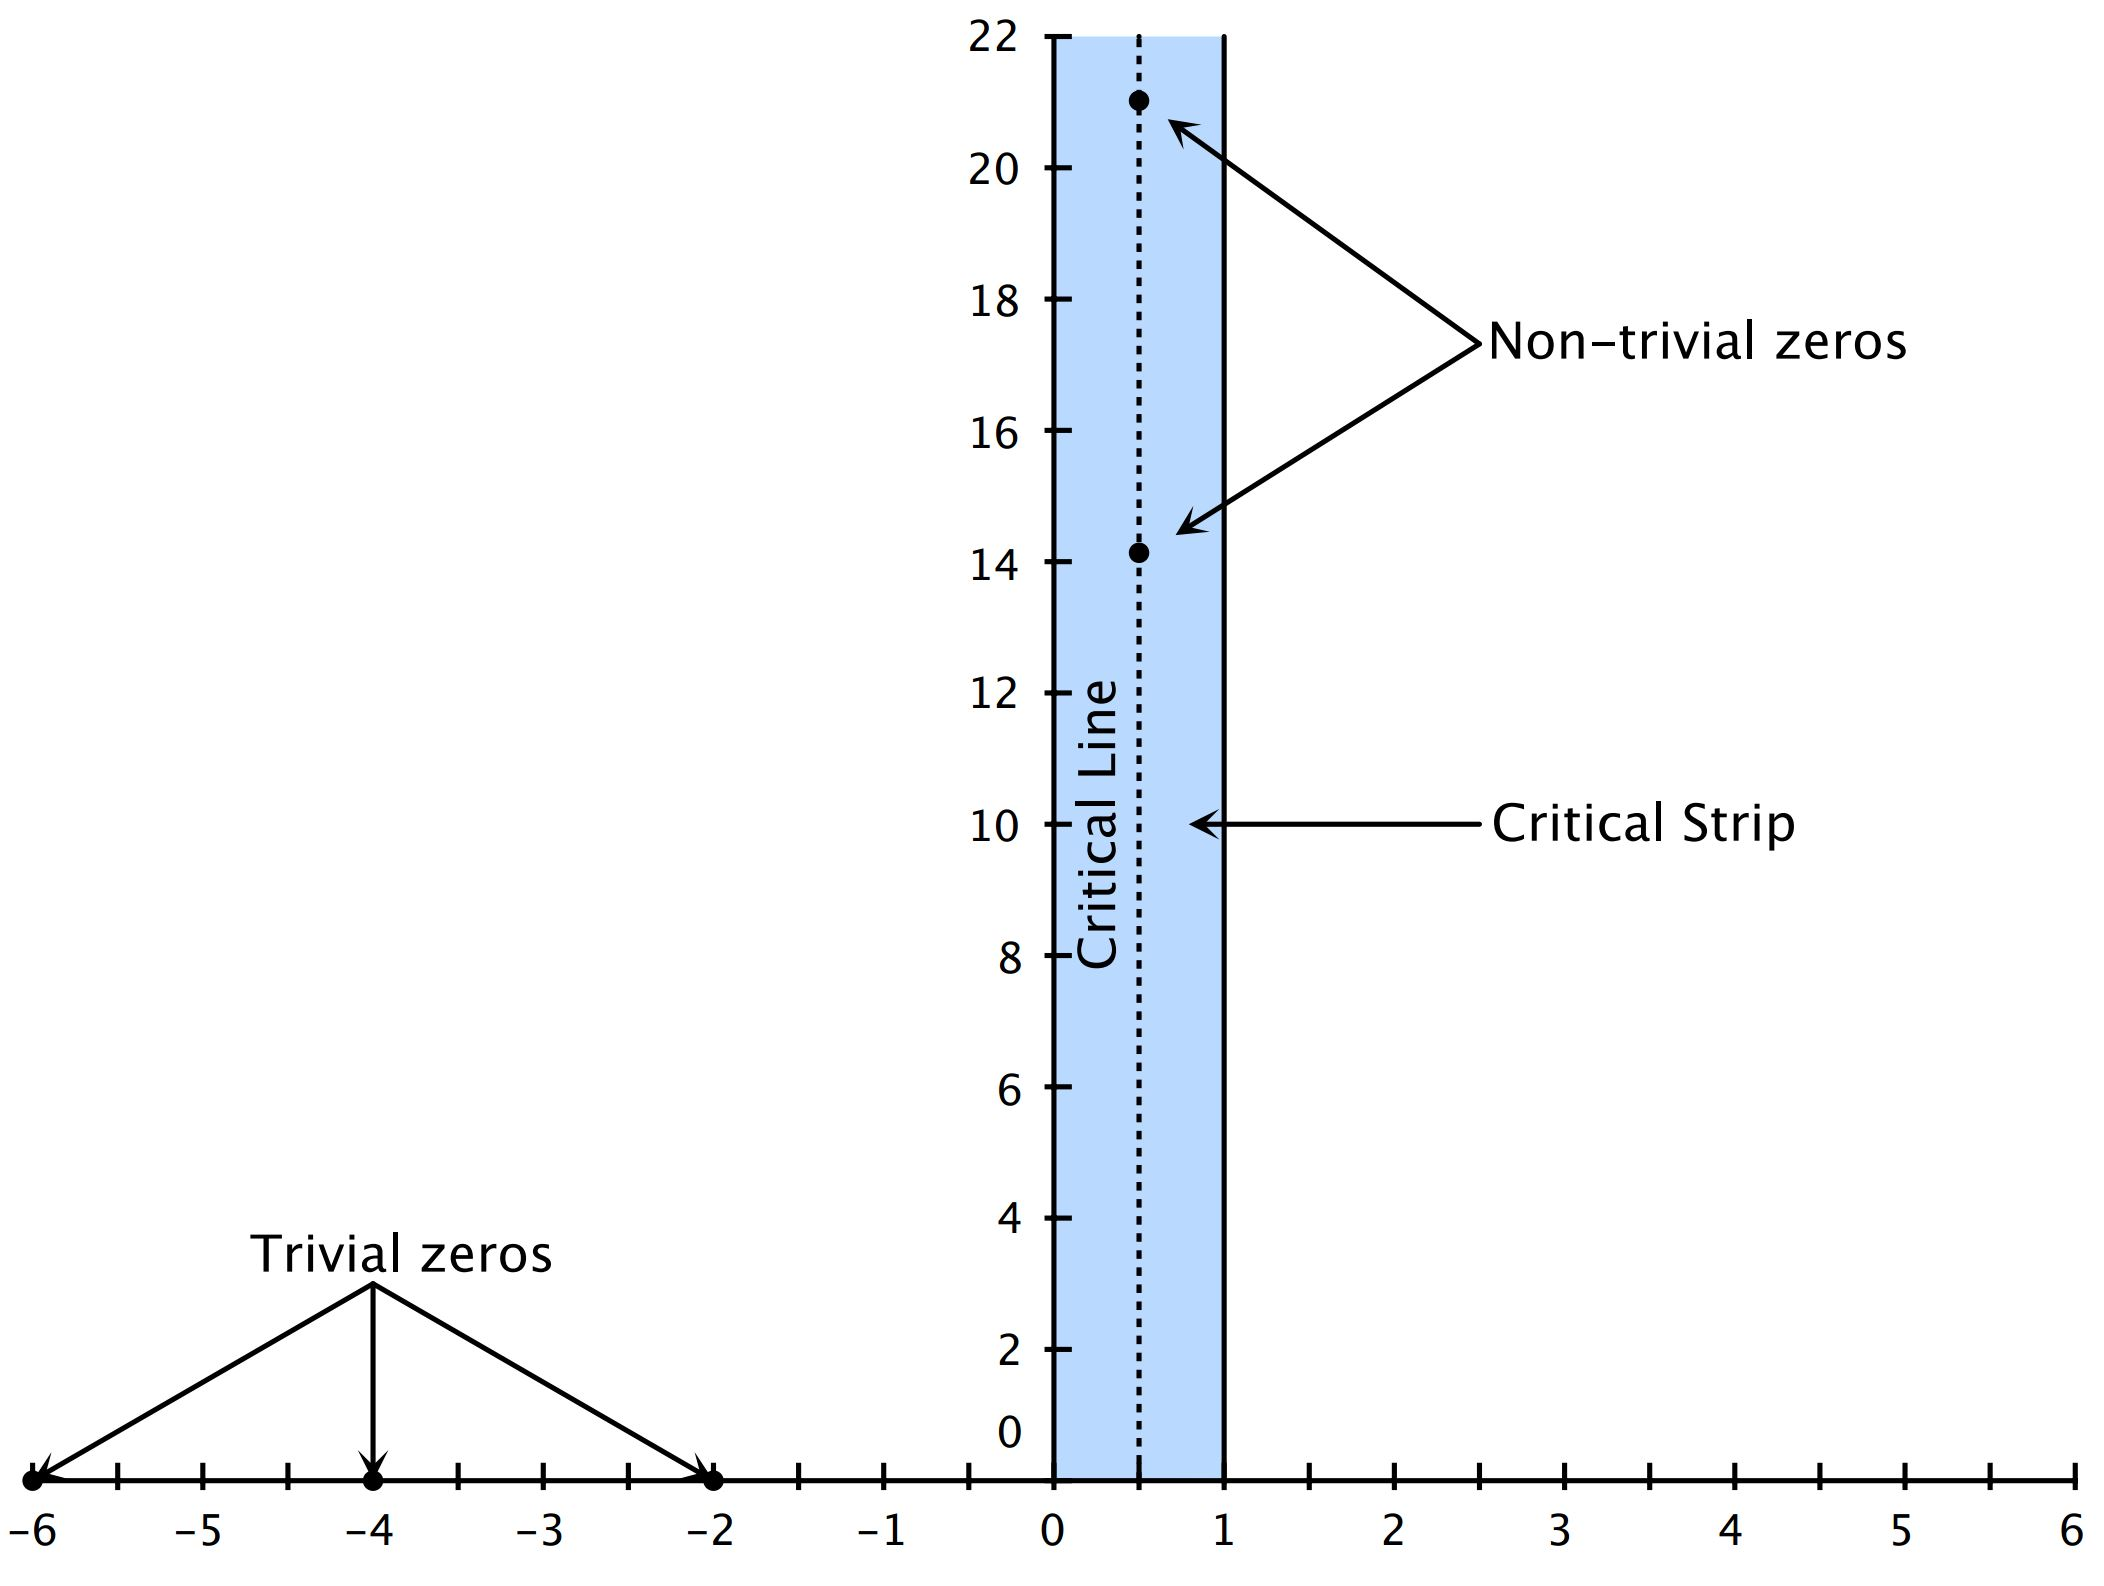
\includegraphics[scale=0.15]{Riemann.JPG}
        \caption{Hipótesis de Riemann\footnotemark{}.}
    \end{figure}
    \vspace{-7mm}\footnotetext{\bibentry{RH}}
\end{frame}

\section{CRIPTOGRAFÍA MODERNA}
\subsection{Generalidades}
\begin{frame}{CRIPTOGRAFÍA MODERNA}
\framesubtitle{Generalidades}
	\begin{itemize}
      \item No se intercambian el mensaje clave, doble candado.
      \item Primos grandes
      \item Eficiencia computacional
      	\begin{equation*}
      		O((\log n)^{c\log\log\log n})
      	\end{equation*}
        \begin{equation*}
        	O(e^{\sqrt{c\log n(\log\log n)^2}})
        \end{equation*}
      \item Atkin, Sundaram, Eratosthenes \vspace{0.35cm}\footnote{\bibentry{Sieve}}
	\end{itemize}
    \begin{figure}
    	\centering
        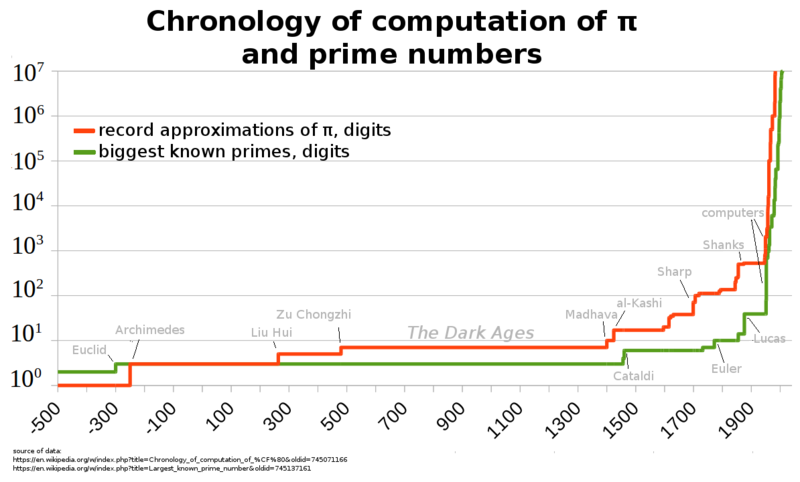
\includegraphics[scale=0.2]{chrono.png}
        \caption{Cronología de pi y los primos a través de los años\footnotemark{}.}
    \end{figure}
    \footnotetext{\bibentry{chrono}}
    \vspace{-12mm}
\end{frame}
%%%%%%%%%%%%%%%%%%%%%%%%%%%%%%%%%%%%%%%%%%%%%%%%%%%%%%%%%%%%%%%%
\subsection{Algoritmo RSA}
\begin{frame}{CRIPTOGRAFÍA MODERNA}
\framesubtitle{Algoritmo RSA}
	\begin{itemize}
	\item 1978, \textbf{R}ivest, \textbf{S}hamir \& \textbf{A}dleman.
    \item Asimétrico.
    \item Multiplicar números es sencillo, factorizarlos es difícil
	\end{itemize}
    Algoritmo: $K_U = (e,n)$, $K_R = (d,n)$
    \begin{enumerate}
    \item $p,q$ primos
    \item $n = pq$
    \item $z = (p-1)(q-1)$
    \item $e$ tal que $e$ primo, $1<e<z$ y $\texttt{GCD}(n,e) = 1$
    \item $d$ tal que $(d \cdot e) \equiv 1 \pmod{z}$
    \end{enumerate}
    Si $m$ es el mensaje original y $c$ el mensaje encriptado, entonces
    \begin{equation*}
    	c = m^e\hspace{2pt}\text{mod}\hspace{2pt} n
    \end{equation*}
    \begin{equation*}
    	m = c^d\hspace{2pt}\text{mod}\hspace{2pt} n
    \end{equation*}
\end{frame}
%%%%%%%%%%%%%%%%%%%%%%%%%%%%%%%%%
\subsection{Ejemplo RSA}
\begin{frame}{CRIPTOGRAFÍA MODERNA}
	\framesubtitle{Ejemplo RSA}
    \begin{itemize}
    \item $p=61$
    \item $q=53$
    \item $n=pq=3233$
    \item $z=(p-1)(q-1)$
    \item $e = 17$
    \item $d = 2753$
    \end{itemize}
    Tenemos $R_U = (e,n)=(17,3233)$, $R_K = (d,n) = (2753,3233)$
    Si tenemos $m = 123$, entonces
    \begin{equation*}
    	c = (123)^{17}\hspace{2pt}\text{mod}\hspace{2pt} 3233 = 855
  	\end{equation*}
    Y si se quiere descifrar,
    \begin{equation*}
    	m = (855)^{2753}\hspace{2pt}\text{mod}\hspace{2pt} 3233 = 123
    \end{equation*}
\end{frame}

\nonumb % Not numbered titles
%\addcontentsline{toc}{section}{\small\protect\numberline{}{REFERENCIAS BIBLIOGRÁFICAS}} % Separated from other contents, for small number of contents
\addcontentsline{toc}{section}{\small REFERENCES} % Closer from other contents, for large number of contents
\nocite{*} % All citations showed (take care with fraud!)
%%%%%%%%%%%%%%%%%%%%%%%%%%%%%%%%%%%%%%%%%%%%%%%%%%%%%%%%%%%%%%%%%%%%%%%%%%%%
\section*{REFERENCES}
\begin{frame}[allowframebreaks]{REFERENCES} %  and put before {REFEREN...}
\begingroup % Group for changing the color
\renewcommand{\color}[1]{} % Allows to have black bibs and white footnote bibs
\small{\bibliographystyle{IEEEtran}} % Size of text; acm or gatech-thesis or ieeetr or ieeetran or icontec or iso690
\bibliography{ref}
\endgroup % Group for changing the color
% pdflatex -> bibtex -> pdflatex -> pdflatex
\end{frame}
%%%%%%%%%%%%%%%%%%%%%%%%%%%%%%%%%%%%%%%%%%%%%%%%%%%%%%%%%%%%%%%%%%%%%%%%%%%%
% Thank-slide
\begin{frame}[plain,noframenumbering] % No frame number
	\begin{beamercolorbox}[ht=\paperheight,wd=\paperwidth, center]{Portada}
		\begin{center}\Huge\textbf{Thank you}\end{center} % Or Thanks; leave the next space mandatorily
		
		\vspace{0.44\paperheight}
    \end{beamercolorbox}
\end{frame}
%%%%%%%%%%%%%%%%%%%%%%%%%%%%%%%%%%%%%%%%%%%%%%%%%%%%%%%%%%%%%%%%%%%%%%%%%%%%


\end{document}
